\documentclass{article}

\usepackage[margin=1in]{geometry}
\usepackage{graphicx, float, tikz}

\title{CS 132 Bonus Homework}

\author{Jason Cheng}

\date{}

\begin{document}
\maketitle

\section*{Q1 A.}

\begin{verbatim}
grammar mydsl.MyDsl with org.eclipse.xtext.common.Terminals

generate myDsl "http://www.MyDsl.mydsl"

Package:
	'package' name=ID '{' members+=Member* '}';

Member:
	Package | User;

User:
	Class | Enum;

Class:
	'class' name=ID ('(' super=[Class|FQN] ')')? ':' attributes+=Attribute*;

Attribute:
	name=ID ':' type=Type;

Enum:
	'enum' name=ID ':' literals+=Literal+;

Literal:
	name=ID '=' symbol=STRING;

FQN:
	ID ('.' ID)*;

Type:
	Builtin | Ref | List | Set;

Builtin:
	t='str' | t='bool';

Ref:
	t=[User|FQN];

List:
	'List' '(' t=[User|FQN] ')';

Set:
	'Set' '(' t=[User|FQN] ')';
\end{verbatim}

\section*{Q1 B.}

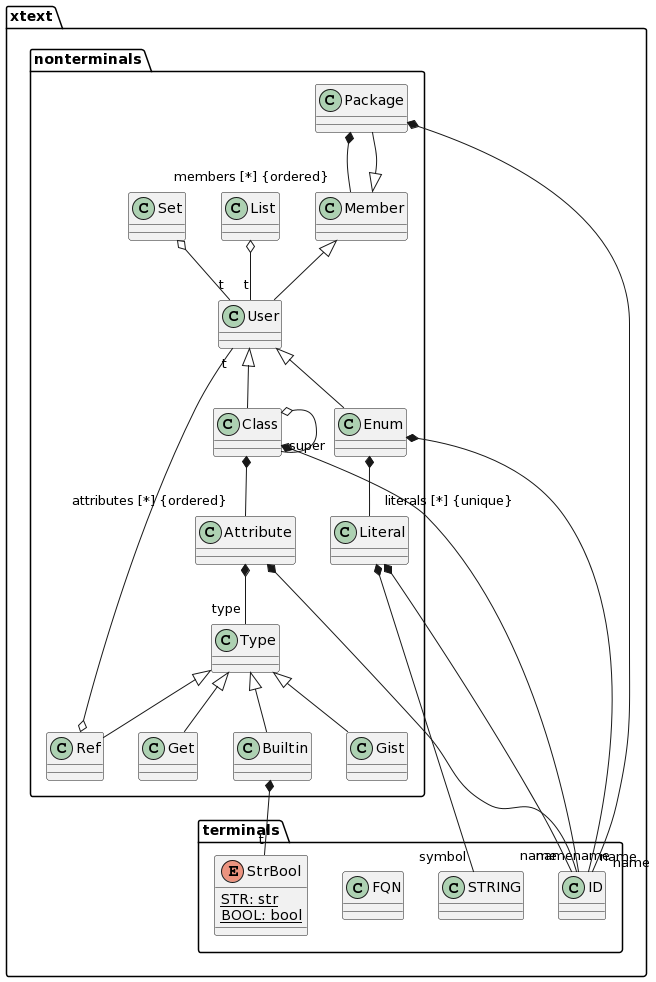
\includegraphics[scale=0.6]{xtext-diagram.png}

\section*{Q2}

\begin{verbatim}
package mydsl.generator

import org.eclipse.emf.ecore.resource.Resource
import org.eclipse.xtext.generator.AbstractGenerator
import org.eclipse.xtext.generator.IFileSystemAccess2
import org.eclipse.xtext.generator.IGeneratorContext

import mydsl.myDsl.Attribute
import mydsl.myDsl.Builtin
import mydsl.myDsl.Class
import mydsl.myDsl.Enum
import mydsl.myDsl.List
import mydsl.myDsl.Literal
import mydsl.myDsl.Member
import mydsl.myDsl.Package
import mydsl.myDsl.Ref
import mydsl.myDsl.Set
import mydsl.myDsl.User
import java.util.Optional

class Names {
    val (String) => String path;
    val (Object) => Optional<String> lookup;

    new((String) => String p,
        (Object) => Optional<String> f) {
        path = p;
        lookup = f;
    }

    def setPath((String) => String p) {
        new Names(p, lookup)
    }

    def addLookup((Object) => Optional<String> f) {
        new Names(path, [o | f.apply(o).or([lookup(o)])])
    }

    def path(String s) {
        path.apply(s)
    }

    def lookup(Object o) {
        lookup.apply(o)
    }
}

class Comp {
    public val String body;
    public val String epilogue;

    new(String b, String ep) {
        body = b;
        epilogue = ep;
    }

    def addBody(String s) {
        new Comp(body + s, epilogue)
    }

    def update((Comp) => Comp f) {
        f.apply(this)
    }

    def addEpilogue(String s) {
        new Comp(body, epilogue + s)
    }

    def export() {
        "@startuml\n"
        + "!pragma useIntermediatePackages false\n"
        + body + epilogue
        + "@enduml\n"
    }
}

class MyDslGenerator extends AbstractGenerator {

    override void doGenerate(Resource resource, IFileSystemAccess2 fsa, IGeneratorContext context) {
        val prgm = resource.contents.filter(Package).head;
        val res = prgm.resolve(new Names([p | p], [Optional.empty]));
        val comp = prgm.compile(res, new Comp("", ""));
        fsa.generateFile('diagram.uml', comp.export());
    }

    def dispatch Names resolve(Package n, Names e) {
        val path = e.path(n.name);
        val e1 = e.setPath([s | path + "." + s]);
        n.members.fold(e1, [es, m | m.resolve(es)]).setPath([s | e.path(s)])
    }

    def dispatch resolve(Member n, Names e) {
        val path = e.path(n.name);
        e.addLookup([o | Optional.of(path).filter([o === n])])
    }

    def dispatch Comp compile(Package n, Names e, Comp o) {
        n.members.fold(o, [os, m | m.compile(e, os)])
    }

    def dispatch Comp compile(Class n, Names e, Comp o) {        
        val path = e.lookup(n).get;

        val o1 = o.addBody(String.format("class %s {\n", path))
            .update([a | n.attributes.fold(a, [os, m | m.compile(e, path, os)])])
            .addBody("}\n");

        val sup = n.getSuper;

        if (sup === null)
            o1
        else
            o1.addEpilogue(String.format("%s <|-- %s\n", e.lookup(sup).get, path))
    }

    def dispatch Comp compile(Enum n, Names e, Comp o) {
        o.addBody(String.format("enum %s {\n", e.lookup(n).get))
            .update([a | n.literals.fold(a, [os, m | m.compile(os)])])
            .addBody("}\n");
    }

    def compile(Attribute n, Names e, String path, Comp o) {
        n.type.compile(
            [String s | o.addBody(String.format("%s: %s\n", n.name, s))],
            [User u, String f | o.addEpilogue(String.format(f, path, n.name, e.lookup(u).get))]
        )
    }

    def compile(Literal n, Comp o) {
        o.addBody(String.format("%s: %s {static}\n", n.name, n.symbol))
    }

    def dispatch compile(Builtin n, (String) => Comp field, (User, String) => Comp arrow) {
        field.apply(n.t)
    }

    def dispatch compile(Ref n, (String) => Comp field, (User, String) => Comp arrow) {
        arrow.apply(n.t, "%s *-- \"%s\" %s\n")
    }

    def dispatch compile(List n, (String) => Comp field, (User, String) => Comp arrow) {
        arrow.apply(n.t, "%s *-- \"%s [*] {ordered}\" %s\n")
    }

    def dispatch compile(Set n, (String) => Comp field, (User, String) => Comp arrow) {
        arrow.apply(n.t, "%s *-- \"%s [*] {unique}\" %s\n")
    }
}
\end{verbatim}

\end{document}
